%%%%%%%%%%%%%%%%%%%%%%%%%%%%%%%%%%%%%%%%%
% 
% Lake Eagles 3761 Poster Template
%
%%%%%%%%%%%%%%%%%%%%%%%%%%%%%%%%%%%%%%%%%

%----------------------------------------------------------------------------------------
%	PACKAGES AND OTHER DOCUMENT CONFIGURATIONS
%----------------------------------------------------------------------------------------

\documentclass[a0,landscape]{a0poster}

%% Macros for Fitch-style natural deduction. 
% Author: Peter Selinger, University of Ottawa
% Created: Jan 14, 2002
% Modified: Feb 8, 2005
% Version: 0.5
% Copyright: (C) 2002-2005 Peter Selinger
% Filename: fitch.sty
% Documentation: fitchdoc.tex
% URL: http://quasar.mathstat.uottawa.ca/~selinger/fitch/

% License:
%
% This program is free software; you can redistribute it and/or modify
% it under the terms of the GNU General Public License as published by
% the Free Software Foundation; either version 2, or (at your option)
% any later version.
%
% This program is distributed in the hope that it will be useful, but
% WITHOUT ANY WARRANTY; without even the implied warranty of
% MERCHANTABILITY or FITNESS FOR A PARTICULAR PURPOSE. See the GNU
% General Public License for more details.
%
% You should have received a copy of the GNU General Public License
% along with this program; if not, write to the Free Software Foundation, 
% Inc., 59 Temple Place, Suite 330, Boston, MA 02111-1307, USA.

% USAGE EXAMPLE:
% 
% The following is a simple example illustrating the usage of this
% package.  For detailed instructions and additional functionality, see
% the user guide, which can be found in the file fitchdoc.tex.
% 
% \[
% \begin{nd}
%   \hypo{1}  {P\vee Q}   
%   \hypo{2}  {\neg Q}                         
%   \open                              
%   \hypo{3a} {P}
%   \have{3b} {P}        \r{3a}
%   \close                   
%   \open
%   \hypo{4a} {Q}
%   \have{4b} {\neg Q}   \r{2}
%   \have{4c} {\bot}     \ne{4a,4b}
%   \have{4d} {P}        \be{4c}
%   \close                             
%   \have{5}  {P}        \oe{1,3a-3b,4a-4d}                 
% \end{nd}
% \]

{\chardef\x=\catcode`\*
\catcode`\*=11
\global\let\nd*astcode\x}
\catcode`\*=11

% References

\newcount\nd*ctr
\def\nd*render{\expandafter\ifx\expandafter\nd*x\nd*base\nd*x\the\nd*ctr\else\nd*base\ifnum\nd*ctr<0\the\nd*ctr\else\ifnum\nd*ctr>0+\the\nd*ctr\fi\fi\fi}
\expandafter\def\csname nd*-\endcsname{}

\def\nd*num#1{\nd*numo{\nd*render}{#1}\global\advance\nd*ctr1}
\def\nd*numopt#1#2{\nd*numo{$#1$}{#2}}
\def\nd*numo#1#2{\edef\x{#1}\mbox{$\x$}\expandafter\global\expandafter\let\csname nd*-#2\endcsname\x}
\def\nd*ref#1{\expandafter\let\expandafter\x\csname nd*-#1\endcsname\ifx\x\relax%
  \errmessage{Undefined natdeduction reference: #1}\else\mbox{$\x$}\fi}
\def\nd*noop{}
\def\nd*set#1#2{\ifx\relax#1\nd*noop\else\global\def\nd*base{#1}\fi\ifx\relax#2\relax\else\global\nd*ctr=#2\fi}
\def\nd*reset{\nd*set{}{1}}
\def\nd*refa#1{\nd*ref{#1}}
\def\nd*aux#1#2{\ifx#2-\nd*refa{#1}--\def\nd*c{\nd*aux{}}%
  \else\ifx#2,\nd*refa{#1}, \def\nd*c{\nd*aux{}}%
  \else\ifx#2;\nd*refa{#1}; \def\nd*c{\nd*aux{}}%
  \else\ifx#2.\nd*refa{#1}. \def\nd*c{\nd*aux{}}%
  \else\ifx#2)\nd*refa{#1})\def\nd*c{\nd*aux{}}%
  \else\ifx#2(\nd*refa{#1}(\def\nd*c{\nd*aux{}}%
  \else\ifx#2\nd*end\nd*refa{#1}\def\nd*c{}%
  \else\def\nd*c{\nd*aux{#1#2}}%
  \fi\fi\fi\fi\fi\fi\fi\nd*c}
\def\ndref#1{\nd*aux{}#1\nd*end}

% Layer A

% define various dimensions (explained in fitchdoc.tex):
\newlength{\nd*dim} 
\newdimen\nd*depthdim
\newdimen\nd*hsep
\newdimen\ndindent
\ndindent=1em
% user command to redefine dimensions
\def\nddim#1#2#3#4#5#6#7#8{\nd*depthdim=#3\relax\nd*hsep=#6\relax%
\def\nd*height{#1}\def\nd*thickness{#8}\def\nd*initheight{#2}%
\def\nd*indent{#5}\def\nd*labelsep{#4}\def\nd*justsep{#7}}
% set initial dimensions
\nddim{4.5ex}{3.5ex}{1.5ex}{1em}{1.6em}{.5em}{2.5em}{.2mm}

\def\nd*v{\rule[-\nd*depthdim]{\nd*thickness}{\nd*height}}
\def\nd*t{\rule[-\nd*depthdim]{0mm}{\nd*height}\rule[-\nd*depthdim]{\nd*thickness}{\nd*initheight}}
\def\nd*i{\hspace{\nd*indent}} 
\def\nd*s{\hspace{\nd*hsep}}
\def\nd*g#1{\nd*f{\makebox[\nd*indent][c]{$#1$}}}
\def\nd*f#1{\raisebox{0pt}[0pt][0pt]{$#1$}}
\def\nd*u#1{\makebox[0pt][l]{\settowidth{\nd*dim}{\nd*f{#1}}%
    \addtolength{\nd*dim}{2\nd*hsep}\hspace{-\nd*hsep}\rule[-\nd*depthdim]{\nd*dim}{\nd*thickness}}\nd*f{#1}}

% Lists

\def\nd*push#1#2{\expandafter\gdef\expandafter#1\expandafter%
  {\expandafter\nd*cons\expandafter{#1}{#2}}}
\def\nd*pop#1{{\def\nd*nil{\gdef#1{\nd*nil}}\def\nd*cons##1##2%
    {\gdef#1{##1}}#1}}
\def\nd*iter#1#2{{\def\nd*nil{}\def\nd*cons##1##2{##1#2{##2}}#1}}
\def\nd*modify#1#2#3{{\def\nd*nil{\gdef#1{\nd*nil}}\def\nd*cons##1##2%
    {\advance#2-1 ##1\advance#2 1 \ifnum#2=1\nd*push#1{#3}\else%
      \nd*push#1{##2}\fi}#1}}

\def\nd*cont#1{{\def\nd*t{\nd*v}\def\nd*v{\nd*v}\def\nd*g##1{\nd*i}%
    \def\nd*i{\nd*i}\def\nd*nil{\gdef#1{\nd*nil}}\def\nd*cons##1##2%
    {##1\expandafter\nd*push\expandafter#1\expandafter{##2}}#1}}

% Layer B

\newcount\nd*n
\def\nd*beginb{\begingroup\nd*reset\gdef\nd*stack{\nd*nil}\nd*push\nd*stack{\nd*t}%
  \begin{array}{l@{\hspace{\nd*labelsep}}l@{\hspace{\nd*justsep}}l}}
\def\nd*resumeb{\begingroup\begin{array}{l@{\hspace{\nd*labelsep}}l@{\hspace{\nd*justsep}}l}}
\def\nd*endb{\end{array}\endgroup}
\def\nd*hypob#1#2{\nd*f{\nd*num{#1}}&\nd*iter\nd*stack\relax\nd*cont\nd*stack\nd*s\nd*u{#2}&}
\def\nd*haveb#1#2{\nd*f{\nd*num{#1}}&\nd*iter\nd*stack\relax\nd*cont\nd*stack\nd*s\nd*f{#2}&}
\def\nd*havecontb#1#2{&\nd*iter\nd*stack\relax\nd*cont\nd*stack\nd*s\nd*f{\hspace{\ndindent}#2}&}
\def\nd*hypocontb#1#2{&\nd*iter\nd*stack\relax\nd*cont\nd*stack\nd*s\nd*u{\hspace{\ndindent}#2}&}

\def\nd*openb{\nd*push\nd*stack{\nd*i}\nd*push\nd*stack{\nd*t}}
\def\nd*closeb{\nd*pop\nd*stack\nd*pop\nd*stack}
\def\nd*guardb#1#2{\nd*n=#1\multiply\nd*n by 2 \nd*modify\nd*stack\nd*n{\nd*g{#2}}}

% Layer C

\def\nd*clr{\gdef\nd*cmd{}\gdef\nd*typ{\relax}}
\def\nd*sto#1#2#3{\gdef\nd*typ{#1}\gdef\nd*byt{}%
  \gdef\nd*cmd{\nd*typ{#2}{#3}\nd*byt\\}}
\def\nd*chtyp{\expandafter\ifx\nd*typ\nd*hypocontb\def\nd*typ{\nd*havecontb}\else\def\nd*typ{\nd*haveb}\fi}
\def\nd*hypoc#1#2{\nd*chtyp\nd*cmd\nd*sto{\nd*hypob}{#1}{#2}}
\def\nd*havec#1#2{\nd*cmd\nd*sto{\nd*haveb}{#1}{#2}}
\def\nd*hypocontc#1{\nd*chtyp\nd*cmd\nd*sto{\nd*hypocontb}{}{#1}}
\def\nd*havecontc#1{\nd*cmd\nd*sto{\nd*havecontb}{}{#1}}
\def\nd*by#1#2{\ifx\nd*x#2\nd*x\gdef\nd*byt{\mbox{#1}}\else\gdef\nd*byt{\mbox{#1, \ndref{#2}}}\fi}

% multi-line macros
\def\nd*mhypoc#1#2{\nd*mhypocA{#1}#2\\\nd*stop\\}
\def\nd*mhypocA#1#2\\{\nd*hypoc{#1}{#2}\nd*mhypocB}
\def\nd*mhypocB#1\\{\ifx\nd*stop#1\else\nd*hypocontc{#1}\expandafter\nd*mhypocB\fi}
\def\nd*mhavec#1#2{\nd*mhavecA{#1}#2\\\nd*stop\\}
\def\nd*mhavecA#1#2\\{\nd*havec{#1}{#2}\nd*mhavecB}
\def\nd*mhavecB#1\\{\ifx\nd*stop#1\else\nd*havecontc{#1}\expandafter\nd*mhavecB\fi}
\def\nd*mhypocontc#1{\nd*mhypocB#1\\\nd*stop\\}
\def\nd*mhavecontc#1{\nd*mhavecB#1\\\nd*stop\\}

\def\nd*beginc{\nd*beginb\nd*clr}
\def\nd*resumec{\nd*resumeb\nd*clr}
\def\nd*endc{\nd*cmd\nd*endb}
\def\nd*openc{\nd*cmd\nd*clr\nd*openb}
\def\nd*closec{\nd*cmd\nd*clr\nd*closeb}
\let\nd*guardc\nd*guardb

% Layer D

% macros with optional arguments spelled-out
\def\nd*hypod[#1][#2]#3[#4]#5{\ifx\relax#4\relax\else\nd*guardb{1}{#4}\fi\nd*mhypoc{#3}{#5}\nd*set{#1}{#2}}
\def\nd*haved[#1][#2]#3[#4]#5{\ifx\relax#4\relax\else\nd*guardb{1}{#4}\fi\nd*mhavec{#3}{#5}\nd*set{#1}{#2}}
\def\nd*havecont#1{\nd*mhavecontc{#1}}
\def\nd*hypocont#1{\nd*mhypocontc{#1}}
\def\nd*base{undefined}
\def\nd*opend[#1]#2{\nd*cmd\nd*clr\nd*openb\nd*guard{#1}#2}
\def\nd*close{\nd*cmd\nd*clr\nd*closeb}
\def\nd*guardd[#1]#2{\nd*guardb{#1}{#2}}

% Handling of optional arguments.

\def\nd*optarg#1#2#3{\ifx[#3\def\nd*c{#2#3}\else\def\nd*c{#2[#1]{#3}}\fi\nd*c}
\def\nd*optargg#1#2#3{\ifx[#3\def\nd*c{#1#3}\else\def\nd*c{#2{#3}}\fi\nd*c}

\def\nd*five#1{\nd*optargg{\nd*four{#1}}{\nd*two{#1}}}
\def\nd*four#1[#2]{\nd*optarg{0}{\nd*three{#1}[#2]}}
\def\nd*three#1[#2][#3]#4{\nd*optarg{}{#1[#2][#3]{#4}}}
\def\nd*two#1{\nd*three{#1}[\relax][]}

\def\nd*have{\nd*five{\nd*haved}}
\def\nd*hypo{\nd*five{\nd*hypod}}
\def\nd*open{\nd*optarg{}{\nd*opend}}
\def\nd*guard{\nd*optarg{1}{\nd*guardd}}

\def\nd*init{%
  \let\open\nd*open%
  \let\close\nd*close%
  \let\hypo\nd*hypo%
  \let\have\nd*have%
  \let\hypocont\nd*hypocont%
  \let\havecont\nd*havecont%
  \let\by\nd*by%
  \let\guard\nd*guard%
  \def\ii{\by{$\Rightarrow$I}}%
  \def\ie{\by{$\Rightarrow$E}}%
  \def\Ai{\by{$\forall$I}}%
  \def\Ae{\by{$\forall$E}}%
  \def\Ei{\by{$\exists$I}}%
  \def\Ee{\by{$\exists$E}}%
  \def\ai{\by{$\wedge$I}}%
  \def\ae{\by{$\wedge$E}}%
  \def\ai{\by{$\wedge$I}}%
  \def\ae{\by{$\wedge$E}}%
  \def\oi{\by{$\vee$I}}%
  \def\oe{\by{$\vee$E}}%
  \def\ni{\by{$\neg$I}}%
  \def\ne{\by{$\neg$E}}%
  \def\be{\by{$\bot$E}}%
  \def\nne{\by{$\neg\neg$E}}%
  \def\r{\by{R}}%
}

\newenvironment{nd}{\begingroup\nd*init\nd*beginc}{\nd*endc\endgroup}
\newenvironment{ndresume}{\begingroup\nd*init\nd*resumec}{\nd*endc\endgroup}

\catcode`\*=\nd*astcode

% End of file fitch.sty



% The name of the package, capitalized or not.
\def\QT{\textsf{\emph{Qtree}}}
\def\Qt{\textsf{\emph{qtree}}}
\def\pstyle#1{\textsf{#1}} % style filenames
\def\argplain#1{\textit{$\langle$#1$\rangle$}} % Like \marg, but without { }

\usepackage{qtree}

\usepackage{multicol} % This is so we can have multiple columns of text side-by-side
\columnsep=100pt % This is the amount of white space between the columns in the poster
\columnseprule=3pt % This is the thickness of the black line between the columns in the poster

\usepackage[svgnames]{xcolor} % Specify colors by their 'svgnames', for a full list of all colors available see here: http://www.latextemplates.com/svgnames-colors

\usepackage{hyperref}

%\usepackage{times} % Use the times font
\usepackage{palatino} % Uncomment to use the Palatino font

\usepackage{graphicx} % Required for including images
\graphicspath{{figures/}} % Location of the graphics files
\usepackage{booktabs} % Top and bottom rules for table
\usepackage[font=small,labelfont=bf]{caption} % Required for specifying captions to tables and figures
\usepackage{amsfonts, amsmath, amsthm, amssymb} % For math fonts, symbols and environments
\usepackage{wrapfig} % Allows wrapping text around tables and figures

\usepackage{tikz}
\usetikzlibrary{graphs}

\begin{document}
%----------------------------------------------------------------------------------------
%	POSTER HEADER 
%----------------------------------------------------------------------------------------

\begin{minipage}[b]{0.55\linewidth}
\veryHuge \color{NavyBlue} \textbf{Lake Eagles \#3761} \color{Black}\\ % Title
\Huge\textit{ Playbook }\\[1cm] % Subtitle
\huge \textbf{
Food \& Beverages \\ 
Bar, Keno \& Pull-tabs Drawers\\
Maintenance }\\ % Author(s)
\end{minipage}
%
\begin{minipage}[b]{0.25\linewidth}
\color{DarkSlateGray}\Large \textbf{Contact Information}\\
Lake Eagles Aerie \# 3761 FOE\\ % Address
8460 W. Ludington Drive \\
Lake, MI 48632 \\
Phone: 989-544-3761 \\ % Phone number
Website: \texttt{https://3761.mifoe.com/}\\ % Email address
\end{minipage}
%
\begin{minipage}[b]{0.19\linewidth}

\includegraphics[width=12cm]{./FOE.png} % Logo or a photo of you, adjust its dimensions here
\end{minipage}

\vspace{1cm} % A bit of extra whitespace between the header and poster content

%----------------------------------------------------------------------------------------

\begin{multicols}{4} % This is how many columns your poster will be broken into, a poster with many figures may benefit from less columns whereas a text-heavy poster benefits from more

%----------------------------------------------------------------------------------------
%	ABSTRACT
%----------------------------------------------------------------------------------------

\color{Navy} % Navy color for the abstract
%
\begin{abstract}
\textsc{NOTE:} It is important (in my opinion) to work cooperatively. This means we work as a team and each of us needs to work from the same play-book. What follows is our playbook as I now understand it. The playbook needs to constant revision so that it contains all the necessary information that would be sufficient to continue operations at Lake Eagles \#3761.

\vspace{.5cm}

\begin{flushright}
Thanks, the editor.
\end{flushright}

\end{abstract}

%----------------------------------------------------------------------------------------
%	Food and Beverage 
%----------------------------------------------------------------------------------------

\color{SaddleBrown} % SaddleBrown color for the introduction

\section*{Food: Menu and Regular Specials}

Our menu will inevitably change, but when it does it requires planning and careful thought. A small change to the menu may require changes to our weekly routine, our suppliers, and a learning curve in which waste and costs increase. 

\vspace{.5cm}

\begin{flushright}
Make changes thoughtfully $\hdots$ just saying.
\end{flushright}

\subsection*{Menu}
\begin{center}
\begin{tabular}{ l r l r}
Grilled Cheese & \$2.00 & Mozzarella Sticks & \$4.00 \\
Grilled Cheese w/ ham & \$4.00 & Jalapeño Poppers & \$4.50 \\
Hot Dog & \$2.50 & Mushrooms & \$4.50 \\
Coney Dog & \$3.00 & Cauliflower & \$4.50 \\
Fish Sandwich & \$4.50 & Onion Rings & \$3.00 \\
Chicken Strips & \$5.25 & French Fries & \$2.50 \\
Chicken Sandwich & \$4.50 & Curly Fries & \$2.50 \\
Wing Dings & \$4.75 & Tater Tots & \$2.50 \\
Popcorn Chicken & \$4.25 & &\\
Hamburger & \$4.00 & (50 cents off on baskets) & \\
Hamburger w/ cheese & \$4.50 & & \\
Dbl Hamburger & \$6.00 & & \\
Dbl Hamburger w/ cheese & \$6.50 & & \\
Philly Cheese Steak & \$5.00 & & \\
Boneless Wings & \$5.00 & & \\
\end{tabular}
\end{center}

\subsection*{Mexican Wednesday}

\begin{center}
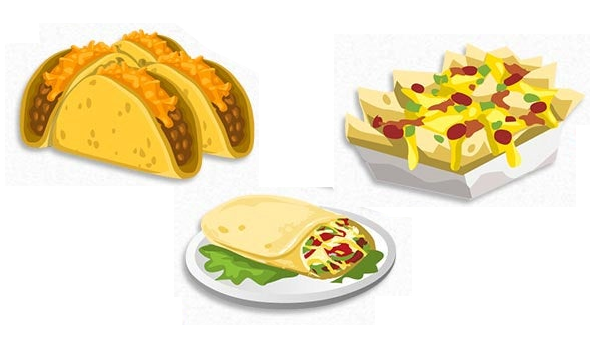
\includegraphics[width=0.8\linewidth]{images/mexican1}
%\captionof{figure}{\color{Green} Mexican Night}
\end{center}

\vspace{.5cm}

\begin{center}
\begin{tabular}{ l r }
Wet Burrito & \$7.50 \\
Taco Salad in edible bowl & \$7.50 \\
Nacho Plate & \$7.50 \\
Taco (soft or hard shell) & \$2.00 \\
Chips and Salsa & \$3.00 \\
\end{tabular}
\end{center}

\vspace{1cm}

All meals include lettuce, onion, green pepper, tomato and shredded cheese. Sour cream, salsa (hot,med,mild), and jalapeno available on request.


\subsection*{Fish Friday}

\begin{center}

\includegraphics[width=0.8\linewidth]{images/fishfry}
%\captionof{figure}{\color{Green} Mexican Night}
\end{center}

\begin{center}
\begin{tabular}{ l r }
Cup of Soup & \$2.00 \\ 
Soup and Salad Bar & \$7.00 \\
3-Piece Cod Dinner (1/2 lb) & \$9.00 \\
All-You-Can-Eat Cod Dinner & \$11.00 \\
10-Piece Bluegill Dinner (1/2 lb) & \$11.00 \\
3-Piece Walleye Dinner (3/4 lb) & \$11.00 \\
8-Piece Shrimp Dinner (1/2 lb) & \$9.00 \\
Shrimp / Cod Combo Dinner & \$9.00 \\
Seafood Platter & \$15.00 \\
\end{tabular}
\end{center}

\vspace{.5cm}

All dinners include choice of potato and our soup and salad bar.

%----------------------------------------------------------------------------------------
%	Beverages
%----------------------------------------------------------------------------------------

\color{DarkSlateGray} % DarkSlateGray color for the rest of the content

\section*{Beverages}
\begin{center}


\includegraphics[width=0.8\linewidth]{images/beer_kegs}
%\captionof{figure}{\color{Green} Mexican Night}
\end{center}

\begin{center}
\begin{tabular}{ l r }
16oz Draft & \$1.25 \\
24oz Draft & \$2.00 \\
Cold Pitcher & \$5.00 \\
Domestic Beer & \$2.00 \\
Domestic Bucket (6 cans) & \$10.00 \\
Corona & \$2.50 \\
Ciderboys & \$2.50 \\
Wine & \$2.75 \\
Coffee & \$0.50 \\
Bottled Water & \$1.00 \\
Iced Tea & \$1.00 \\
Juice & \$1.00 \\
Pop & \$1.25 \\
\end{tabular}
\end{center}

\vspace{1cm}

\noindent \textsc{Draft Beer} \\
Budweiser, Bud Light, Miller Lite, \& Busch Light \\

\noindent \textsc {Canned Beer} \\
Busch Light, Budweiser, Bud Light, Miller Lite, Miller High Life, Miller Select 64, Coors Light, Michelob Ultra, Michelob Light, PBR, Corona Light, \& Corona Extra. \\

\noindent \textsc{Top Shelf Liquor} \\

\begin{center}
\begin{tabular}{ l l r }

Top Shelf & &\$3.50 \\
\hline
& & \\
Jack Daniels & Whiskey &\\
Jim Beam & Whiskey &\\
Crown Royal & Whiskey &\\
Maker's Mark & Whiskey &\\
J \& B & Whiskey & \\
Tito's & Vodka &\\
UV Blue & Vodka &\\
Jos\'e Cuervo & Tequilla & \\
& & \\
\hline
\end{tabular}
\end{center}

\vspace{.5cm}

\noindent \textsc{Mid Shelf Liquor} \\
\begin{center}
\begin{tabular}{ l l r }
Mid Shelf & &\$2.75 \\
\hline
Captain Morgan & & \\
Canadian Mist & Whiskey & \\
Canadian Club & Whiskey & \\
Christian Brothers & Brandy & \\
Bacardi & Rum & \\
Bacardi L\'imon & Rum & \\
Seagram's 7 & Whiskey & \\
Seagram's VO & Whiskey & \\

& & \\
Bottom Shelf & &\$2.50 \\
\hline
Mohawk & Vodka & \\
Lauder's & Scotch & \\
Gordon's & Gin & \\
Old Crow & & \\
Black Velvet & & \\
Kessler's & & \\

\hline
\end{tabular}
\end{center}

Christian Brother's Brandy, Gordon's Gin, Amaretto, Blackberry Brandy, Buttershots, Cranberry, Ginger, Grape Pucker, Kahlua, Kessler, Midori Melon Liqueur, Peachtree, Peppermint Schnapps, Sloe Gin, Bacardi, Bacardi Limon, Captain Morgan, Malibu Rum, Lauder's Scotch, Jose Cuervo, Mohawk Vodka, Tito's Vodka, UV Blue Vodka, Black Velvet, Canadian Club, Canadian Mist, Crown Royal, Crown Royal Apple, J\&B, Jack Daniels, Jack Daniels Fire, Jameson, Jim Beam, Jim Beam Red Stag, Maker's Mark, McMaster's Canadian, Old Crow, Seagram's 7, Seagram’s VO, Southern Comfort,

\vspace{1cm}

\textsc{Wines \& Coolers}


%----------------------------------------------------------------------------------------
%	Supplier: Food
%----------------------------------------------------------------------------------------

\color{DarkGreen}
\section*{Suppliers: Food}
\begin{center}


\includegraphics[width=0.8\linewidth]{images/gfs}
%\captionof{figure}{\color{Green} Mexican Night}
\end{center}

\subsection*{Gordon's Food Service}
We have an account at \textsc{Gordon's Food Service} (GFS) and order the following items on a weekly basis as needed.

\vspace{0.5cm}

\begin{center}
\begin{tabular}{ l l r }
\hline
\# & Item & Price \\
\hline
414601 & French Fries 6/case & \$24.46\\
324167 & Tator Tots 6/case & \$44.99\\
181501 & Curly Fries 6/case & \$41.38\\
267100 & Onion Rings 6/case & \$37.46 \\
694570 & Breaded Mushrooms 6/case  & \$37.01 \\
714303 & Breaded Mozzarella Sticks 1/case & \$54.53 \\
 & Breaded Cauliflower & \\
 & Jalape\~no Poppers & \\
 
\hline
\end{tabular}
\end{center}

\subsection*{Produce and Groceries}

%----------------------------------------------------------------------------------------
%	Bartender: Daily
%----------------------------------------------------------------------------------------

\color{Navy}
\section*{Bartender Daily}


\subsection*{Opening Routine}

\begin{itemize}
\item Unlock main entrance and disarm alarm. 
\item Turn on lights and Keno monitors. 
\item Check bathroom paper towels, toilet paper and trash. 
\item Fill ice caddie at bar and add ice to urinals. 
\item Shelve bar glasses. 
\item Put dishes in strainer away. 
\item Wash dishes that have been soaking overnight. 
\item Pick up trash, clean table and chairs. 
\item Stock pop, beer, liquor, and mixers. 
\item Inventory pop and add to Meijer's weekly list. 
\item Inventory mixers and add to Gordon's weekly list. 
\item Cut lemon and lime if needed. 
\item Count Keno drawer, cash register drawer, pull tab drawer, and bank bag. 
\item Sign On Keno machine. (See code under the drawer.) 
\item "Start the Day" on the cash register. (one cash no sale). 
\item Turn on "Open" signs. 
\item Unlock porch. 
\item Turn on Fryer and Hood fan.
\end{itemize}


\subsection*{Closing Routine}
\begin{itemize}
\item Turn off Fryer and Hood fan. 
\item Turn off Oven and Grill and clean. 
\item Do pickup around bar. Combine trash. 
\item Do bar dishes. 
\item Put away bar supplies. Dump open pop. 
\item Stock Pop and canned beer. 
\item Wipe down taps and sinks. 
\item Wipe down tables, bar counter and chairs. 
\item Vacuum carpet. 
\item Turn off Open signs / replace with Closed. 
\item Close all freezer and refrigerator doors. 
\item Note any low supplies. Stock Kitchen supplies per prep list. 
\item Do dishes in kitchen. 
\item Collect food trash. 
\item Clean Kitchen Surfaces. 
\item Sweep and mop kitchen. 
\item Clean toilets / urinals. 
\item Clean sinks and mirrors. 
\item Check toilet paper, soap, paper towels 
\item Collect All Trash and take out to dumpster. 
\item Count and record bank bag. 
\item Count and record pull tab drawer. 
\item Run Keno report for today. 
\item Count and record Keno drawer. Paperclip winning tickets, Keno report, and money. Place bundle in drawer. 
\item Run cash register reports. (See codes under drawer.) 
\item Count and record cash register drawer. 
\item Put today's take into the Day Bag. Paperclip report, money, and take sheet. Place bundle in Day Bag. 
\item Place money bags in safe inside the lock box. 
\item Place money drawers in safe along with The Daily and The Weekly. 
\item Close and lock safe. Scramble combination. 
\item Turn off Keno boards and TV. 
\item Lock Porch. 
\item Turn off lights. 
\item Arm alarm and exit building. 
\end{itemize}



\color{DarkSlateGrey}
\section*{Suppliers \& Inventory}


\section*{Mathematical Section}

Nulla vel nisl sed mauris auctor mollis non sed. 

\begin{equation}
E = mc^{2}
\label{eqn:Einstein}
\end{equation}

Curabitur mi sem, pulvinar quis aliquam rutrum. (1) edf (2)
, $\Omega=[-1,1]^3$, maecenas leo est, ornare at. $z=-1$ edf $z=1$ sed interdum felis dapibus sem. $x$ set $y$ ytruem. 
Turpis $j$ amet accumsan enim $y$-lacina; 
ref $k$-viverra nec porttitor $x$-lacina. 

Vestibulum ac diam a odio tempus congue. Vivamus id enim nisi:

\begin{eqnarray}
\cos\bar{\phi}_k Q_{j,k+1,t} + Q_{j,k+1,x}+\frac{\sin^2\bar{\phi}_k}{T\cos\bar{\phi}_k} Q_{j,k+1} &=&\nonumber\\ 
-\cos\phi_k Q_{j,k,t} + Q_{j,k,x}-\frac{\sin^2\phi_k}{T\cos\phi_k} Q_{j,k}\label{edgek}
\end{eqnarray}
and
\begin{eqnarray}
\cos\bar{\phi}_j Q_{j+1,k,t} + Q_{j+1,k,y}+\frac{\sin^2\bar{\phi}_j}{T\cos\bar{\phi}_j} Q_{j+1,k}&=&\nonumber \\
-\cos\phi_j Q_{j,k,t} + Q_{j,k,y}-\frac{\sin^2\phi_j}{T\cos\phi_j} Q_{j,k}.\label{edgej}
\end{eqnarray} 

Nulla sed arcu arcu. Duis et ante gravida orci venenatis tincidunt. Fusce vitae lacinia metus. Pellentesque habitant morbi. $\mathbf{A}\underline{\xi}=\underline{\beta}$ Vim $\underline{\xi}$ enum nidi $3(P+2)^{2}$ lacina. Id feugain $\mathbf{A}$ nun quis; magno. Fusce convallis rutrum turpis, quis aliquet enim accumsan id. Vestibulum ullamcorper porttitor convallis. Integer sagittis interdum malesuada. Class aptent taciti sociosqu ad litora torquent per conubia nostra, per inceptos himenaeos. Sed adipiscing tristique orci at ullamcorper. Morbi accumsan, urna et porttitor pulvinar, lacus risus dignissim massa. Proin sollicitudin. Pellentesque eget orci eros. Fusce ultricies, tellus et pellentesque fringilla, ante massa luctus libero, quis tristique purus urna nec nibh.

%----------------------------------------------------------------------------------------
%	RESULTS 
%----------------------------------------------------------------------------------------

\section*{Results}

Donec faucibus purus at tortor egestas eu fermentum dolor facilisis. Maecenas tempor dui eu neque fringilla rutrum. Mauris \emph{lobortis} nisl accumsan. Aenean vitae risus ante. Pellentesque condimentum dui. Etiam sagittis purus non tellus tempor volutpat. Donec et dui non massa tristique adipiscing.
%
\begin{wraptable}{l}{12cm} % Left or right alignment is specified in the first bracket, the width of the table is in the second
\begin{tabular}{l l l}
\toprule
\textbf{Treatments} & \textbf{Response 1} & \textbf{Response 2}\\
\midrule
Treatment 1 & 0.0003262 & 0.562 \\
Treatment 2 & 0.0015681 & 0.910 \\
Treatment 3 & 0.0009271 & 0.296 \\
\bottomrule
\end{tabular}
\captionof{table}{\color{Green} Table caption}
\end{wraptable}
%
Phasellus imperdiet, tortor vitae congue bibendum, felis enim sagittis lorem, et volutpat ante orci sagittis mi. Morbi rutrum laoreet semper. Morbi accumsan enim nec tortor consectetur non commodo nisi sollicitudin. Proin sollicitudin. Pellentesque eget orci eros. Fusce ultricies, tellus et pellentesque fringilla, ante massa luctus libero, quis tristique purus urna nec nibh.

Nulla ut porttitor enim. Suspendisse venenatis dui eget eros gravida tempor. Mauris feugiat elit et augue placerat ultrices. Morbi accumsan enim nec tortor consectetur non commodo. Pellentesque condimentum dui. Etiam sagittis purus non tellus tempor volutpat. Donec et dui non massa tristique adipiscing. Quisque vestibulum eros eu. Phasellus imperdiet, tortor vitae congue bibendum, felis enim sagittis lorem, et volutpat ante orci sagittis mi. Morbi rutrum laoreet semper. Morbi accumsan enim nec tortor consectetur non commodo nisi sollicitudin.

\begin{center}\vspace{1cm}

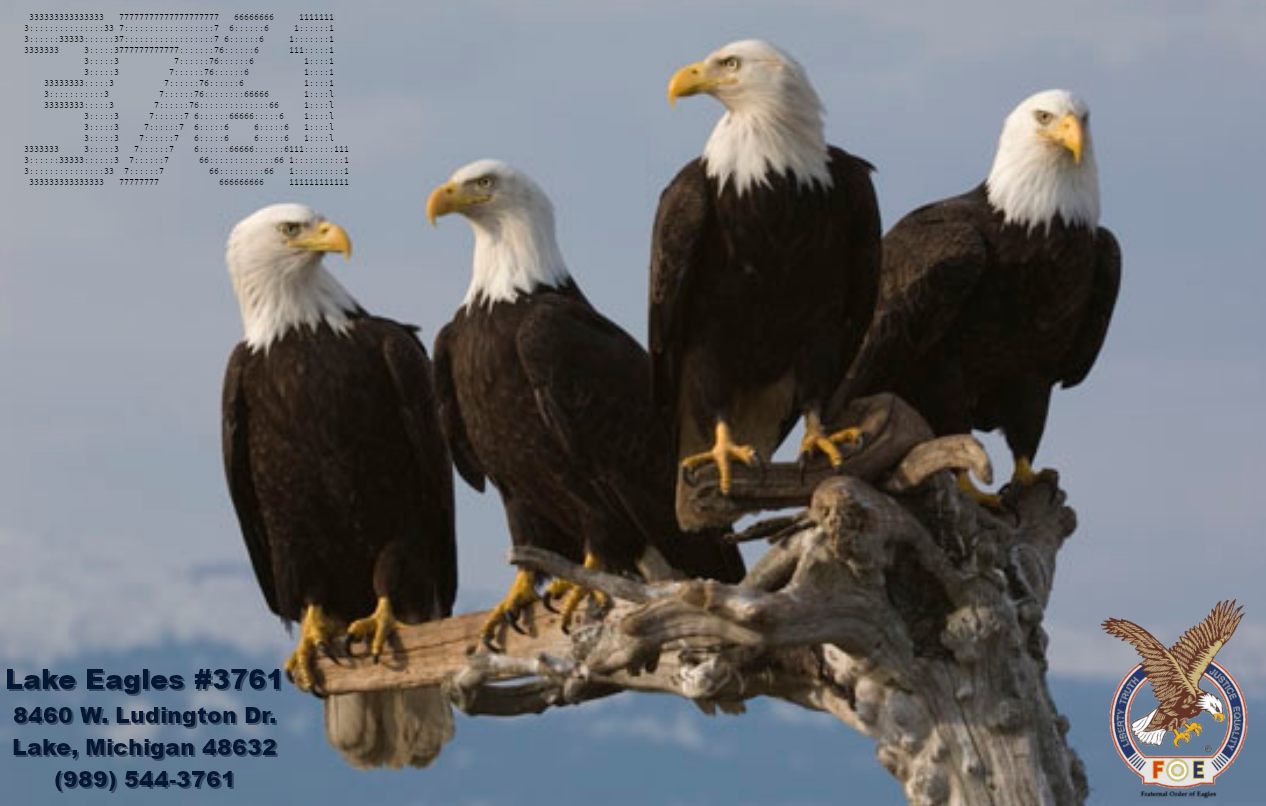
\includegraphics[width=0.8\linewidth]{images/the_club2b}

\captionof{figure}{\color{Green} Figure caption}

\end{center}\vspace{1cm}

In hac habitasse platea dictumst. Etiam placerat, risus ac.

Adipiscing lectus in magna blandit:

\begin{center}\vspace{1cm}
\begin{tabular}{l l l l}
\toprule
\textbf{Treatments} & \textbf{Response 1} & \textbf{Response 2} \\
\midrule
Treatment 1 & 0.0003262 & 0.562 \\
Treatment 2 & 0.0015681 & 0.910 \\
Treatment 3 & 0.0009271 & 0.296 \\
\bottomrule
\end{tabular}
\captionof{table}{\color{Green} Table caption}
\end{center}\vspace{1cm}

Vivamus sed nibh ac metus tristique tristique a vitae ante. Sed lobortis mi ut arcu fringilla et adipiscing ligula rutrum. Aenean turpis velit, placerat eget tincidunt nec, ornare in nisl. In placerat.

\begin{center}\vspace{1cm}
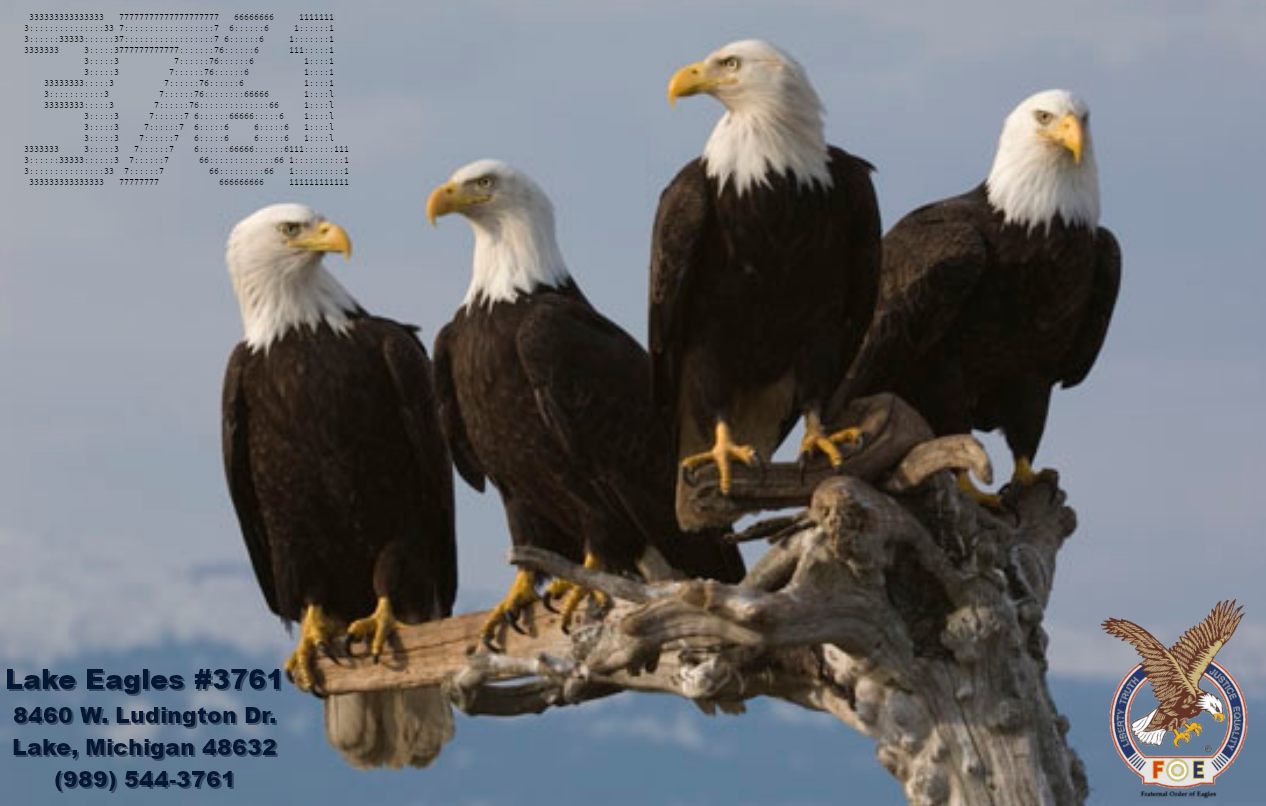
\includegraphics[width=0.8\linewidth]{images/the_club2b}
\captionof{figure}{\color{Green} Figure caption}
\end{center}\vspace{1cm}

%----------------------------------------------------------------------------------------
%	CONCLUSIONS
%----------------------------------------------------------------------------------------

\color{SaddleBrown} % SaddleBrown color for the conclusions to make them stand out

\section*{Conclusions}

\begin{itemize}
\item Pellentesque eget orci eros. Fusce ultricies, tellus et pellentesque fringilla, ante massa luctus libero, quis tristique purus urna nec nibh. Phasellus fermentum rutrum elementum. Nam quis justo lectus.
\item Vestibulum sem ante, hendrerit a gravida ac, blandit quis magna.
\item Donec sem metus, facilisis at condimentum eget, vehicula ut massa. Morbi consequat, diam sed convallis tincidunt, arcu nunc.
\item Nunc at convallis urna. isus ante. Pellentesque condimentum dui. Etiam sagittis purus non tellus tempor volutpat. Donec et dui non massa tristique adipiscing.
\end{itemize}

\color{DarkSlateGray} % Set the color back to DarkSlateGray for the rest of the content

%----------------------------------------------------------------------------------------
%	FORTHCOMING RESEARCH
%----------------------------------------------------------------------------------------

\section*{Forthcoming Research}

Vivamus molestie, risus tempor vehicula mattis, libero arcu volutpat purus, sed blandit sem nibh eget turpis. Maecenas rutrum dui blandit lorem vulputate gravida. Praesent venenatis mi vel lorem tempor at varius diam sagittis. Nam eu leo id turpis interdum luctus a sed augue. Nam tellus.

 %----------------------------------------------------------------------------------------
%	REFERENCES
%----------------------------------------------------------------------------------------

\nocite{*} % Print all references regardless of whether they were cited in the poster or not
\bibliographystyle{plain} % Plain referencing style
\bibliography{sample} % Use the example bibliography file sample.bib

%----------------------------------------------------------------------------------------
%	ACKNOWLEDGEMENTS
%----------------------------------------------------------------------------------------

\section*{Acknowledgements}

Etiam fermentum, arcu ut gravida fringilla, dolor arcu laoreet justo, ut imperdiet urna arcu a arcu. Donec nec ante a dui tempus consectetur. Cras nisi turpis, dapibus sit amet mattis sed, laoreet.

%----------------------------------------------------------------------------------------

\end{multicols}
\end{document}